\documentclass{sig-alternate}
%\usepackage[utf8]{inputenc}
\usepackage[hidelinks]{hyperref}
\usepackage{comment}
\usepackage{array}
\usepackage{url}
\usepackage{listings}
\usepackage{algorithm}
\usepackage{algorithmic}
\newcommand{\redcolor}[1]{\textcolor{red}{#1}}
\newcommand{\bluecolor}[1]{\textcolor{blue}{#1}}
\newcommand{\figref}[1]{Figure~\ref{#1}}
\newcommand{\secref}[1]{Section~\ref{#1}}
\newcommand{\appref}[1]{Appendix~\ref{#1}}
\newcommand{\tabref}[1]{Table~\ref{#1}}
\newcommand{\algoref}[1]{Algorithm~\ref{#1}}
\newcommand\Mark[1]{\textsuperscript#1}
\def\sharedaffiliation{\end{tabular}\newline\begin{tabular}{c}}

% Making caption 9pt; bold face
\usepackage[font=small,labelfont=bf,textfont=bf]{caption}
\captionsetup[table]{skip=6pt}
\captionsetup[figure]{skip=6pt}

\def\iiitd{$^1$}
\def\imperial{$^2$}
\def\southampton{$^3$}
\def\ucla{$^4$}

% specialcell; see http://tex.stackexchange.com/a/19678
\newcommand{\specialcell}[2][c]{%
  \begin{tabular}[#1]{@{}c@{}}#2\end{tabular}}

\usepackage{xcolor}
\usepackage{colortbl}
\usepackage{xfrac}

\hyphenation{AMPds UKPD REDD iAWE HES Smart BLUED}

\title{NILMTK: An Open Source Toolkit for Non-intrusive Load Monitoring}

%\numberofauthors{1}

%\author{
%%	Nipun Batra\iiitd, 
%	Jack Kelly\imperial, 
%	Oliver Parson\southampton, 
%	Haimonti Dutta\iiitd,
%	William Knottenbelt\imperial, 
%	Alex Rogers\southampton,
%	Amarjeet Singh\iiitd,
%	Mani B. Srivastava\ucla
%\sharedaffiliation
%  \begin{tabular}{cccc}
%    \affaddr{{\iiitd}Indraprastha Institute of Information Technology{\ }} & \affaddr{{\iiitd}Imperial College{\ }} & \affaddr{{\iiitd}University of Southampton{\ }} & \affaddr{{\ucla}University of California{\ }} \\
%    \affaddr{Delhi, India}                  &{London, UK} &{Southampton, UK} & \affaddr{Los Angeles, United States} \\
%\email{\{nipunb,manojg,amarjeet\}@iiitd.ac.in} & \email{\{jack.kelly,w.knottenbelt\}@imperial.ac.uk} & \email{\{op106,acr\}@ecs.soton.ac.uk}  & mbs@ucla.edu
%  \end{tabular}
%}
\vspace{-2pt}
\author{Nipun Batra$^1$, Jack Kelly$^2$, Oliver Parson$^3$, Haimonti Dutta$^4$, William Knottenbelt$^2$,\\ Alex Rogers$^3$, Amarjeet Singh$^1$, Mani Srivastava$^5$\\ 
\small$^1$Indraprastha Institute of Information Technology Delhi, India ~\{nipunb,~amarjeet\}@iiitd.ac.in\\
\small$^2$ Imperial College London ~\{jack.kelly,~wjk\}@imperial.ac.uk\\
\small$^3$ University of Southampton ~\{op106,~acr\}@ecs.soton.ac.uk\\
\small$^4$ CCLS Columbia ~\{haimonti@ccls.columbia.edu\}\\
\small$^5$ UCLA ~\{mbs@ucla.edu\}\\
}
%}
%T - number of time slices.

%t - a time slice.

%N - number of appliances.

%n - an appliance.

%K - number of states.

%k - an appliance state.

%\bar{y}^_t - measured aggregate power in time slice t.

%y^{(n)}_t - ground truth power of appliance n in time slice t.

%\hat{y}^{(n)}_t - estimated power of appliance n in time slice t.

%x(n)t - ground truth state of appliance n in time slice t.

%x^(n)t - estimated state of appliance n in time slice t.

\date{January 2014}

\begin{document}

\maketitle

%\begingroup
%\centering
%{\LARGE The Title \\[1.5em]
%\large First Author\Mark{1}, Second Author\Mark{2}, Third Author\Mark{1}, Fourth Author\Mark{2} and Fifth %Author\Mark{3}}\\[1em]
%\begin{tabular}{*{3}{>{\centering}p{.25\textwidth}}}
%\Mark{1}Department1 & \Mark{2}Department2 & \Mark{3}Department3 \tabularnewline
%School1 & School2 & School3 \tabularnewline
%\url{email1} & \url{email2} & \url{email3}
%\end{tabular}\par
%\endgroup


\begin{abstract}
\noindent
\textit{
Non-intrusive load monitoring, or energy disaggregation, aims to separate household energy consumption data collected from a single point of measurement into appliance-level consumption data. In recent years, the field has rapidly expanded due to increased interest as national deployments of smart meters have begun in many countries. However, empirically comparing disaggregation algorithms is currently virtually impossible. This is due to the different data sets used, the lack of reference implementations of these algorithms and the variety of accuracy metrics employed. To address this challenge, we present the Non-intrusive Load Monitoring Toolkit~(NILMTK); an open source toolkit designed specifically to enable the comparison of energy disaggregation algorithms in a reproducible manner. This work is the first research to compare multiple disaggregation approaches across multiple publicly available data sets. Our toolkit includes parsers for a range of existing data sets, a set of statistics for describing data sets, two reference benchmark disaggregation algorithms and a suite of accuracy metrics. We demonstrate the range of reproducible analyses which are made possible by our toolkit, including the analysis of six publicly available data sets and the evaluation of both benchmark disaggregation algorithms across such data sets.
%that our toolkit makes it easier to enter into energy disaggregation research by simplifying the use of multiple data sets, while supporting the addition of new disaggregation algorithms, and also encouraging direct comparisons to be made between algorithms through common accuracy metrics.
}
\end{abstract}

\section{Introduction}

\noindent
Non-intrusive load monitoring (NILM), or energy disaggregation, aims to break down a household's aggregate electricity consumption into individual appliances~\cite{hart_1992}. The motivations for such a process are threefold. First, informing a household's occupants of how much energy each appliance consumes empowers them to take steps towards reducing their energy consumption~\cite{darby_2006}. Second, personalised feedback can be provided which quantifies the savings of certain appliance-specific advice, such as the financial savings when an old inefficient appliance is replaced by a new efficient appliance. Third, if the NILM system is able to determine the time of use of each appliance, a recommender system would be able to inform the household's occupants of the savings of deferring appliance use to a time of day when electricity is either cheaper or has a lower carbon footprint.
%TO DISCUSS: do we also want to mention benefits of disaggregation for utility companies (they can do a better job of forecasting demand / managing the grid) and governments (easier to do large appliance usage surveys)?

Such benefits have drawn significant interest in the field since its inception 25 years ago. In recent years, the combination of smart meter meter deployments~\cite{CaliforniaPublicUtilitiesCommission2006,DepartmentofEnergy&ClimateChange2013} and reduced hardware costs of household electricity sensors has led to a rapid expansion of the field. Such rapid growth over the past 5 years has been evidenced by the wealth of academic papers published, international meetings held (e.g.\ NILM 2012\footnote{\url{http://www.ices.cmu.edu/psii/nilm/}} and EPRI NILM 2013\footnote{\url{http://goo.gl/dr4tpq}}), startup companies founded (e.g. Bidgely and Neurio) and data sets released, (e.g.\ REDD~\cite{redd}, BLUED~\cite{blued} and Smart*~\cite{smart}).

However, three core obstacles currently prevent the direct comparison of state-of-the-art approaches, and as a result may be impeding progress within the field. To the best of our knowledge, each contribution to date has only been evaluated on a single data set and consequently it is hard to assess whether such approaches generalise to new households. Furthermore, many researchers sub-sample data sets to select specific households, appliances and time periods, making experimental results more difficult to reproduce. Second, newly proposed approaches are rarely compared against the same benchmark algorithms, further increasing the difficulty in empirical comparisons of performance between different publications. Moreover, the lack of reference implementations of these state-of-the-art algorithms often leads to the reimplementation of such approaches. Third, many papers target different use cases for NILM and therefore the accuracy of their proposed approaches are evaluated using a different set of performance metrics. As a result the numerical performance calculated by such metrics cannot be compared between any two papers. These three obstacles have led to the proposal of successive extensions to state-of-the-art algorithms, while a direct comparison between new and existing approaches remains impossible.

Similar obstacles have arisen in other research fields and prompted the development of toolkits specifically designed to support research in that area. For example, PhysioToolkit offers access to over 50 databases of physiological data and provides software to support the processing and analysis of such data for the biomedical research community~\cite{physionet}. Similarly, CRAWDAD collects 89 data sets of wireless network data in addition to software to aid the analysis of such data for the wireless network community~\cite{crawdad}. However, no such toolkit is available to the NILM community.

Against this background, we propose NILMTK\footnote{Code: \url{http://github.com/nilmtk/nilmtk}}; an open source toolkit designed specifically to enable easy access to and comparative analysis of energy disaggregation algorithms across diverse data sets. NILMTK provides a complete pipeline from data sets to accuracy metrics, thereby lowering the entry barrier for researchers to implement a new algorithm and compare its performance against the current state of the art. NILMTK has been:
\begin{itemize}
\item released as open source software (with documentation\footnote{Documentation: \url{http://nilmtk.github.io/nilmtk}}) in an effort to encourage researchers to contribute data sets, benchmark algorithms and accuracy metrics as they are proposed, with the goal of enabling a greater level of collaboration within the community. 
\item designed using a modular structure, therefore allowing researchers to reuse or replace individual components as required. The API design is influenced by \texttt{scikit-learn}~\cite{scikit}, which is a machine learning library in Python, well known for its consistent API and complete documentation.
\item written in Python with flat file input and output formats, in addition to high performance binary formats, ensuring compatibility with existing algorithms written in any language and designed for any platform.
\end{itemize}

%\bluecolor{I think your contribution is NILMTK which has these sub-components. Each of them as a standalone probably does not deem fit as a contribution. Especially considering the space constraint you may chop this as well or restrict it to a few sentences. }
The contributions of NILMTK are summarised as follows:
\begin{itemize}
\item We propose NILMTK-DF (data format), the standard energy disaggregation data structure used by our toolkit.  NILMTK-DF is modelled loosely on the REDD data set format~\cite{redd} to allow easy adoption with the community. Furthermore, we provide parsers from six existing data sets into our proposed NILMTK-DF format. 
\item We provide statistical and diagnostic functions which provide a detailed understanding of each data set.  We also provide preprocessing functions for mitigating common challenges with NILM data sets.
\item We provide implementations of two benchmark disaggregation algorithms: first an approach based on combinatorial optimisation~\cite{hart_1992}, and second an approach based on the factorial hidden Markov model~\cite{redd,kim_2011}. We demonstrate the ease by which NILMTK allows the comparison of these algorithms across a range of existing data sets, and present results of their performance.
\item We present a suite of accuracy metrics which are able to evaluate the performance of any disaggregation algorithm which produces an output compatible with NILMTK. This allows the performance of a disaggregation algorithm to be evaluated for a range of use cases.
\end{itemize}

The remainder of this paper is organised as follows. In \secref{sec:related} we provide an overview of related work. In \secref{sec:nilmtk} we present NILMTK and describe its components. In \secref{evaluation} we demonstrate the empirical evaluations which are enabled by NILMTK, and provide analyses of existing data sets and disaggregation algorithms. Finally, in \secref{sec:conclusions} we conclude the paper and propose directions for future work.

\section{Background}
\label{sec:related}

\begin{table*}[]
  \centering
  \begin{tabular}{c c c c c c c c}
    \hline
    \bf Data set & \bf Institution & \bf Location & \bf Duration & \bf Number & \bf Appliance & \bf Aggregate\\
    \bf  & \bf  & \bf  & \bf per  & \bf of & \bf sample & \bf sample\\
    \bf  & \bf  & \bf  & \bf house & \bf houses & \bf frequency & \bf frequency \\
    \hline
    REDD (2011) & MIT & MA, USA & 3-19 days & 6 & 3 sec & 1 sec \& 15 kHz\\
    BLUED (2012) & CMU & PA, USA & 8 days & 1 & N/A* & 12 kHz\\
    Smart* (2012) & UMass & MA, USA & 3 months & 1 & 1 sec & 1 sec\\
    Tracebase (2012) & Darmstadt & Germany & N/A & N/A & 1-10 sec & N/A\\
    Sample (2013) & Pecan Street & TX, USA & 7 days & 10 & 1 min & 1 min\\
    HES (2013) & DECC, DEFRA & UK & 1 or 12 months & 251 & 2 or 10 min
    & 2 or 10 min\\
    AMPds (2013) & Simon Fraser U. & BC, Canada & 1 year & 1 & 1 min & 1 min\\
    iAWE (2013) & IIIT Delhi & Delhi, India & 73 days & 1 & 1 sec & 1 sec\\
    UKPD (2014) & Imperial College & London, UK & 3-14 months & 4 & 6 sec & 1-6 sec \& 16 kHz\\
    \hline
  \end{tabular}
  \caption{Comparison of household energy data sets. *BLUED labels state transitions for each appliance.}
  \label{table:datasets}
\end{table*}

\noindent
The field of non-intrusive load monitoring was founded 25 years ago when Hart proposed the first algorithm for the disaggregation of household energy usage~\cite{hart_1992,armel_2013}. 
%Since then, many studies have shown the benefits of disaggregated data to both household occupants leading to financial savings, and also to utility providers providing demand response management~\cite{zeifman_2011,armel_2013}. 
However, the majority of research prior to 2011 had been evaluated using either lab-based or simulated data and hence the performance of disaggregation algorithms in real households had remained unknown. More recently, national deployments of smart meters have prompted a renewed interest in energy disaggregation. 
%As a result a number of data sets, collected specifically for energy disaggregation have been released. The remainder of this section is organised as follows. 
We now discuss recent research which have contributed new data sets (\secref{sec:datasets}), disaggregation algorithms (\secref{sec:algorithms}) and evaluation metrics (\secref{sec:evaluation_metrics}) to the field. 
%In \secref{sec:datasets} we discuss some of the publicly available data sets. 
%In \secref{sec:algorithms} we discuss discuss recent publications which have
%used such data sets for the evaluation of disaggregation algorithms. 
%In \secref{sec:evaluation_metrics} we discuss the metrics used to compare disaggregation algorithms. 
In \secref{sec:need_nilm_toolkit} we discuss general purpose toolkits, and finally in \secref{sec:notation} we formalise the NILM problem drawing upon notation used in prior literature.

\subsection{Data Sets}
\label{sec:datasets}
\noindent In 2011, the Reference Energy Disaggregation Dataset (REDD)~\cite{redd} was introduced as the first publicly available data set collected specifically to aid NILM research. The data set contains both aggregate and sub-metered power data from 6 households, and has since become the most popular data set for evaluating energy disaggregation algorithms. In 2012, the Building-Level fUlly-labeled dataset for Electricity Disaggregation (BLUED) \cite{blued} was released containing data from a single household. However, the data set does not include sub-metered power data, and instead events triggered by appliance state changes were recorded. 
As a result, it is only possible to evaluate whether changes in appliance states have been detected (e.g.\ washing machine turns on), rather than the assignment of aggregate power demand to individual appliances (e.g.\ washing machine draws 2~kW power). More recently, the Smart*~\cite{smart} data set was released, which contains household aggregate power data from 3 households, while sub-metered appliance power data was only collected from a single household.
%\bluecolor{unclear what is the difference between inferring appliance activity and disaggregation of appliance.}

In 2013 the Pecan Street sample data set was released~\cite{pecan}, which contains both aggregate and sub-metered power data from 10 households. Later, the Household Electricity Survey data set was released~\cite{hes}, which contains data from 251 households although aggregate data was only collected for 14 households. The Almanac of Minutely Power dataset (AMPds)~\cite{ampds} was also released that year containing both aggregate and sub-metered power data from a single household. Subsequently, the Indian data for Ambient Water and Electricity Sensing (iAWE)~\cite{iawe} was released, which contains both aggregate and sub-metered power data from a single house. Most recently, the UK Power Dataset (UKPD) \cite{ukpd} was released which contains data from four households using both aggregate meters and individual appliance sub-meters. Unfortunately, subtle differences in the aims of each data set have led to completely different data formats being used. As a result, a time-consuming engineering barrier exists when using the data sets, each of which are in different formats. This has resulted in publications using only a single data set to evaluate a given approach, and consequently the generality of results over large numbers of households are rarely investigated. We summarise these data sets in \tabref{table:datasets}.

%\bluecolor{you may summarize the literature using different datasets and their differences in a table if you need some more space}
\subsection{Disaggregation Algorithms \& Benchmarks}
\label{sec:algorithms}
\noindent The REDD data set was proposed along with a performance result of a benchmark disaggregation algorithm using 10 second data across 5 of the 6 households~\cite{redd}. Kolter and Jaakkola later proposed an extension to the benchmark algorithm~\cite{kolter_2012}, however the extension was only evaluated using features extracted from 14~kHz data from a single house from the data set, and therefore the performance results are not directly comparable. Later, Zeifman~\cite{zeifman_2012} and Johnson and Willsky~\cite{johnson_2013} evaluated various approaches using the same data set, although both selected a different subset of appliances and calculated an artificial household aggregate from these appliances, therefore simplifying the disaggregation problem and preventing a numerical comparison with other publications. Subsequently, Parson et al.~\cite{parson_2012} and Rahayu et al.~\cite{rahayu_2012} both proposed new approaches, although each were evaluated using a different set of 4 houses from the REDD data set, again preventing a numerical comparison between publications. Last, Batra et al.~\cite{batra_2013} evaluated their approach on the REDD data set using a different household to Kolter and Jaakkola. As a result, it has not been possible to deduce whether one approach is preferable to another from the literature.

The BLUED data set was introduced along with a benchmark algorithm~\cite{blued}, but has since only been used by one other publication~\cite{anderson_2012}. Similarly, AMPds has only been used to evaluate disaggregation algorithms proposed by the data set authors~\cite{ampds}. Clearly, the variety of different formats is slowing the uptake of new data sets, and also preventing algorithms from being tested across multiple data sets. 

It is essential to compare newly proposed disaggregation algorithms to the state of the art in order to assess the increase in an algorithm's performance. However, the lack of available reference implementations of state-of-the-art disaggregation algorithms has led to authors often comparing against more basic benchmark algorithms. This problem is further compounded since there is no single consensus on which benchmarks to use, and as a result most publications use a different benchmark algorithm. For example, Kolter and Jaakkola compared their approach to a set of decoupled HMMs~\cite{kolter_2012}, Parson et al.\ and Batra et al.\ both evaluated their approaches against variants of their own approaches~\cite{parson_2012,batra_2013}, Zeifman compared their approach to a Bayesian classifier, while Rahayu et al. and Johnson and Willsky both compared against a Factorial Hidden Markov Model (FHMM)~\cite{rahayu_2012,johnson_2013}. Clearly, further publications would benefit from openly available benchmark algorithms against which newly proposed algorithms could be easily compared.

%\bluecolor{you could provide a comparison of different evaluation metrics in a table rather than in a text format.}
\subsection{Evaluation metrics}
\label{sec:evaluation_metrics}
\noindent The range of different application areas of energy disaggregation has prompted a number of evaluation metrics to be proposed. For example, four disaggregation metrics labelled \emph{energy correctly assigned} have recently been used to evaluate the performance of disaggregation algorithms using the REDD data set. First, Kolter and Johnson~\cite{redd} proposed an accuracy metric which captures the error in assigned energy normalised by the actual energy consumption in each time slice averaged over all appliances, which was also later used by Rahayu et al.~\cite{rahayu_2012} and Johnson and Willsky~\cite{johnson_2013}. However, large errors in the assigned energy in some time slices will result in a negative accuracy, making this an ill-posed metric. Second, Kolter and Jaakkola~\cite{kolter_2012} proposed an equivalent metric wherein the error is presented individually for each appliance rather than an average across all appliances. Third, Parson et al.~\cite{parson_2012} proposed a metric which captures the error in assigned energy consumed over the complete duration of the data set rather than per time slice. This metric allows overestimates and underestimates in the assigned energy in different time slices to cancel out, and therefore does not represent all disaggregation errors. Fourth, Batra et al.~\cite{batra_2013} proposed a subtly different metric to Kolter and Johnson~\cite{redd}, in which error is reported instead of accuracy, and also energy assigned to an incorrect appliance is double counted as both an overestimate of one appliance's energy consumption and an underestimate of another. The differences between these four metrics prevent numerical comparisons between publications, and motivate the use of common metrics.

\subsection{General Purpose Toolkits}
\label{sec:need_nilm_toolkit}
\noindent Although no toolkit currently exists specifically for energy disaggregation, various toolkits are available for more general machine learning tasks. For example, \texttt{scikit-learn} is a general purpose machine learning toolkit implemented in Python~\cite{scikit} and \texttt{GraphLab} is a machine learning and data mining toolkit written in C++~\cite{graphlab}. While such toolkits provide generic implementations of machine learning algorithms, they lack functionality specific to the energy disaggregation domain, such as data set parsers, benchmark disaggregation algorithms, and energy disaggregation metrics. Therefore, an energy disaggregation toolkit should extend such general toolkits rather than replace them, in a similar way that \texttt{scikit-learn} adds machine learning functionality to the \texttt{numpy} numerical library for Python. 
%This further motivates a toolkit designed specifically for energy disaggregation research.

\subsection{Energy Disaggregation Definition}
\label{sec:notation}
\noindent The aim of energy disaggregation is to provide estimates, $\hat{y}^{(n)}_t$, of the actual power demand, $y^{(n)}_t$, of each appliance $n$ at time $t$, from household aggregate power readings, $\bar{y}_t$. Most NILM algorithms model appliances using a set of discrete states such as off, on, intermediate, etc.  We use $x^{(n)}_t \in \{1, \dots, K\}$ to represent the ground truth state, and $\hat{x}^{(n)}_t$ to represent the appliance state estimated by a disaggregation algorithm.

\section{NILMTK}
\label{sec:nilmtk}

\noindent
We designed NILMTK with two core use cases in mind. First, it should enable the analysis of existing data sets and algorithms. Second, it should provide a simple interface for the addition of new data sets and algorithms.
%\begin{enumerate}
%\item Analysis of existing data sets and algorithms.
%\item Ease of adding new algorithms proposed or new data sets released for broad comparison across existing benchmarks.
%\item Ease of deploying learnt models for processing online as well as offline data.\bluecolor{to reconsider}
%\end{enumerate}
To do so, we implemented NILMTK in Python due to the availability of a vast set of libraries supporting both machine learning research (e.g.\ \texttt{Pandas}, \texttt{scikit-learn}) and the deployment of such research as web applications (e.g.\ \texttt{Django}). Furthermore, Python allows easy deployment in diverse environments including academic settings and is increasingly being used for data science.
% For now not citing the other scikit-learn paper, we should cite this at a later stage!, scikit_api}.

%, which is a well known machine learning framework in the Python community. Scikit-learn is designed for general purpose machine learning tasks and has set high code and documentation standards. However, as discussed earlier in \secref{sec:related}, the domain specifics of NILM demand a specialised framework. 

\figref{fig:pipeline} presents the NILMTK pipeline from the import of data sets to the evaluation of various disaggregation algorithms over various metrics. We discuss each module of the pipeline in the remainder of this section.

\begin{figure*}
\centering 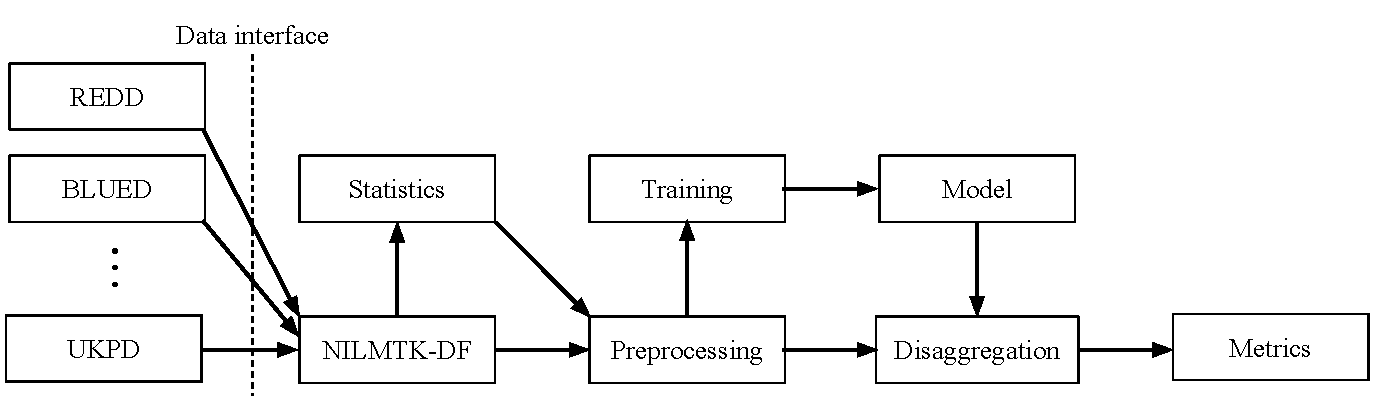
\includegraphics[scale=0.6]{figures/pipeline.pdf}
\caption{NILMTK pipeline. At each stage of the pipeline, results and data can be stored to or loaded from disk.}
\label{fig:pipeline}
\end{figure*}


\subsection{Data Format}%\bluecolor{maybe data interface?}}
\label{sec:data_format} 

\noindent
Motivated by our discussion of the wide differences between multiple data sets released in public domain in \secref{sec:datasets}, we propose NILMTK-DF; a common
data set format inspired by the REDD format~\cite{redd}, into which
existing data sets can be converted. NILMTK currently includes
importers for the following data sets: REDD, Smart*, Pecan Street, iAWE, AMPds
and UKPD. BLUED was excluded due to the lack of sub-metered power data, the Tracebase data set was not included due to the lack of household aggregate power data and HES was not included due to time constraints.
%\bluecolor{Jack has mentioned that HES contains aggregate data from 14 homes!!}

After import, the data resides in our NILMTK-DF in-memory data structure, which is used throughout the NILMTK pipeline. Data can be saved or loaded from disk at multiple stages in the NILMTK processing pipeline to allow other tools to interact with NILMTK.  We provide two CSV flat file formats: a rich NILMTK-DF CSV format and a ``strict REDD" format which allows researchers to use their existing tools designed to process REDD data.  We also provide a more efficient binary format using the Hierarchical Data Format (HDF5).  In addition to storing electricity data, NILMTK-DF can also store relevant metadata and other sensor modalities such as gas, water, temperature, etc. It has been shown that such additional sensor and metadata information may help enhance NILM prediction~\cite{schoofs_2010}. 

Another important feature of our format is the standardisation of nomenclature.  Different data sets use different labels for the same class of appliance (e.g.\ REDD uses `refrigerator' whilst AMPds uses `FGE') and different names for the measured parameters.  When data is first imported into NILMTK, these diverse labels are converted to a standard vocabulary\footnote{\href{https://github.com/nilmtk/nilmtk/blob/master/docs/standard_names/appliances.txt}{\texttt{nilmtk/docs/standard\_names/appliances.txt}}}.

In addition, NILMTK allows rich metadata to be associated with a
household, appliance or meter.  For example, NILMTK can store the
parameters measured by each meter (e.g.\ reactive power, real power),
the geographical coordinates of each house (to enable weather data to be retreived), the mains wiring
defining the meter hierarchy (useful if a single appliance is measured
at the appliance, circuit and aggregate levels), whether a single
meter measures multiple appliances and whether a specific lamp is
dimmable. A full description is provided in
\appref{app:appendix_data_format}.

%% This is interesting and should be there as a motivation!
Through such a combination of metadata and standard nomenclature, NILMTK allows for analysis of appliance data across multiple data sets. For example, users can perform queries such as:
`what is the energy consumption of refrigerators in the USA
compared to the UK?'. Further examples are given in
Appendix~\ref{app:examples}.

We have defined a common interface for data set importers
which, combined with the definition of our in-memory data structures,
enables developers to easily add new data set
importers to NILMTK.

\subsection{Data Set Diagnostics}
\label{sec:diagnostic_definitions}

\noindent
Since no data set is perfect, researchers are required to explore the characteristics of each data set before
disaggregation approaches can be evaluated.  To help diagnose these issues, NILMTK
provides diagnostic functions including:

\textbf{Detect gaps:} Many NILM algorithms assume that each sensor channel is
contiguous. However, this assumption is violated when sensors are off or
malfunctioning.  A `gap' exists between any pair of consecutive
samples if the time elapsed between them is larger than
some threshold.

\textbf{Dropout rate:} The
dropout rate is the total number of recorded samples, divided by the
number of expected samples (which is the length of the time window
under consideration multiplied by the sample rate).

\textbf{Dropout rate (ignoring gaps):} To quantify the rate
at which a wireless sensor drops samples due to radio issues we
 first remove large gaps where the sensor is off and then
 calculate the dropout rate for the remaining contiguous sections.

\textbf{Up-time:}  The up-time is the total time for which a sensor
was recording.  It is the last timestamp, minus the first timestamp,
minus the duration of any gaps.

\textbf{Diagnose:} NILMTK provides a single \texttt{diagnose}
function which checks for all the issues we have encountered.

\subsection{Data Set Statistics}
\label{sec:stats_definitions}

\noindent
Distinct from \emph{diagnostic} statistics, NILMTK also provides
functions for exploring appliance usage, e.g.:

\textbf{Proportion of energy sub-metered:} Data sets rarely sub-meter
every appliance or circuit, and as a result it is useful to quantify the proportion of
total energy measured by sub-metered channels. 
%divided by the total energy measured by the mains channels.\bluecolor{looks too long a sentence} 
Prior to calculating this
statistic, all gaps present in the mains recordings are masked out of
each sub-metered channel, and therefore any additional missing sub-meter data is assumed to
be due to the meter and load being switched off.

\secref{sec:diagnostic_definitions} and \ref{sec:stats_definitions} have described a subset of the diagnostic and
statistical functions in NILMTK.  Further functions are listed
in Appendix~\ref{app:functions} and in the statistics section of the
online documentation.\footnote{
  \url{http://nilmtk.github.io/nilmtk/stats.html}}
%Section~\ref{evaluation} provides results of the statistical functions described above applied to multiple data sets.

\subsection{Preprocessing of Data Sets}
\label{sec:preprocessing}

\noindent
To mitigate the problems  with different data sets, some of which were presented in \secref{sec:diagnostic_definitions}, NILMTK provides several preprocessing functions, including:

\textbf{Downsample:} As seen in \tabref{table:datasets}, the sampling rate of appliance monitors varies
from 0.008~Hz to 15~kHz across the data sets. The downsample preprocessor down-samples data sets to a specified frequency using aggregation functions such as mean, mode and median.

\textbf{Voltage normalisation:} The data sets presented in \tabref{table:datasets} have been
collected from different countries, where voltage fluctuations vary
widely. Batra et al. showed voltage fluctuates from 180-250~V in the
iAWE data set collected in India~\cite{iawe}, while the voltage in the
Smart* data set varies across the range 118-123~V. Hart et al.\ suggested to account for these voltage fluctuations as they can
significantly impact power draw~\cite{hart_1992}. Therefore, NILMTK
provides a voltage normalisation function based on Hart's equation:
\begin{equation}
\textit{Power}_{\textit{normalised}} = 
\left(\frac{\textit{Voltage}_{\textit{nominal}}}{\textit{Voltage}_{\textit{observed}}}\right)^2 
\times \textit{Power}_{\textit{observed}}
\end{equation}
%Figure \redcolor{X} shows the power draw of an air conditioner, before and after voltage normalisation.

\textbf{Top-$k$ appliances}: It is often advantageous to model the top-$k$ energy consuming appliances instead of all appliances for the following three reasons. 
First, the disaggregation of such appliances provides the most value. Second, such appliances contribute the most salient features, and therefore the remaining appliances can be considered to contribute only noise. Third, each additional modelled appliance might contribute significantly to the complexity of the disaggregation task. Therefore, NILMTK provides a function to identify the top-$k$ energy consuming appliances.

%In addition, the memory required by some NILM algorithms is exponential in the number of appliances. Thus, when a large number of appliances are considered, a single centralised model may not fit into memory.
%, thus motivating the need for distributed algorithms. 
%This necessitates the need to include top-$k$ appliances by their contribution which can be in terms of either energy or power. 

NILMTK also provides preprocessing functions for fixing
other common issues with these data sets, such as: (i) interpolating
small periods of missing data when appliance sensors did not report
readings, (ii) filtering out implausible values (such as readings
where observed voltage is more than twice the rated voltage) and (iii)
filtering out appliance data when mains data is missing.

Each data set importer defines a \texttt{preprocess}
function which runs the necessary preprocessing functions to clean
the specific data set. A detailed account of preprocessing functions supported by NILMTK can be found in
\appref{app:functions} and in the online documentation.\footnote{
  \url{http://nilmtk.github.io/nilmtk/preprocessing.html}}

\subsection{Training and Disaggregation Algorithms}
\label{sec:training}
\noindent
NILMTK provides implementations of two common benchmark disaggregation algorithms: combinatorial optimisation (CO) and factorial hidden Markov model (FHMM). CO was proposed by Hart in his seminal work~\cite{hart_1992}, while techniques based on extensions of the FHMM have been proposed more recently~\cite{redd,kim_2011}. The aim of the inclusion of these algorithms is not to present state-of-the-art disaggregation results, but instead to enable new approaches to be compared to well-studied benchmark algorithms without requiring the reimplementation of such algorithms. We now describe these two algorithms.
%It should be highlighted that the intended purpose of these algorithms is only to serve as benchmarks. We do not claim these to give the best results. We would encourage the community to get involved and submit their algorithms to NILMTK. 

\textbf{Combinatorial Optimisation:}
%\bluecolor{1-2 equations will be useful}
CO finds the \textit{optimal} combination of appliance states, which minimises the difference between the sum of the predicted appliance power and the observed aggregate power, subject to a set of appliance models. 
\begin{equation}
\hat{x}^{(n)}_t=\operatorname*{arg min}_{\hat{x}^{(n)}_t}\left|\bar{y}_t-\sum\limits_{n=1}^{N}\hat{y}^{(n)}_t\right|
\end{equation}
Since each time slice is considered as a separate optimisation problem, each time slice is assumed to be independent.
%Its mathematical formulation is given as follows.
%CO assumes time samples to be independent and identically distributed (iid). 
CO resembles the subset sum problem and thus is NP-complete. The complexity of disaggregation for $T$ time slices is $O(TK^N)$, where $N$ is the number of appliances and $K$ is the number of appliance states. Since the complexity of CO is exponential in the number of appliances, the approach is only computationally tractable for a small number of modelled appliances.

\textbf{Factorial Hidden Markov Model:} The power demand of each appliance can be modelled as the observed value of a hidden Markov model (HMM). The hidden component of these HMMs are the states of the appliances. Energy disaggregation involves jointly decoding the power draw of $n$ appliances and hence a factorial HMM~\cite{fhmm} is well suited. A FHMM can be represented by an equivalent HMM in which each state corresponds to a different combination of states of each appliance. Such a FHMM model has three parameters: (i) prior probability ($\pi$) containing $K^N$ entries, (ii) transition matrix ($A$) containing $K^N~*K^N$ or $K^{2N}$ entries, and (iii) emission matrix ($B$) containing $2K^N$ entries. The complexity of exact disaggregation for such a model is $O(TK^{2N})$, and as a result FHMMs scale even worse than CO. From an implementation perspective, even storing (or computing) $A$ for 14 appliances with two states each consumes 8 GB of RAM. Hence, we propose to validate FHMMs on preprocessed data where the top-$k$ appliances are modelled, and appliances contributing less than a given threshold are discarded. However, it should be noted that more efficient pseudo-time algorithms could alternatively be used for inference over both CO and FHMM.

%For algorithms such as FHMMs, modelling relationships amongst consecutive samples is necessary. Thus, NILMTK provides facilities for dividing data into continuous sets for training and testing purposes. Details for adding new algorithms are provided in \appref{app:new_algo}.
For algorithms such as FHMMs, it is necessary to model the relationships amongst consecutive samples. Thus, NILMTK provides facilities for dividing data into continuous sets for training and testing. Details for adding new algorithms are provided in \appref{app:new_algo}.

\subsection{Appliance Model Import and Export}

%\redcolor{I think the argument here should be: benchmark algos require sub-metered data -> sub-metered data is not available in real deployments -> recent training methods have been proposed which do not require sub-metered data -> need an interface between training and disag to support different training methods}

\noindent
Many approaches require sub-metered power data to be collected for training purposes from the same household in which disaggregation is to be performed. However, such data is costly and intrusive to collect, and therefore is unlikely to be available in a large-scale deployment of a NILM system. As a result, recent research has proposed training methods which do not require sub-metered power data to be collected from each household~\cite{kim_2011,parson_2012}. To provide a clear interface between training and disaggregation algorithms, NILMTK provides a Model module which encapsulates the results of the training module required by the disaggregation module. Each implementation of the Model module must provide import and export functions to interface with a JSON file for persistent model storage. NILMTK currently includes importers and exporters for both the FHMM and CO approaches described in \secref{sec:training}.

%Recently, a lot of interest has arisen in deploying live NILM systems, as evidenced by the many startup companies currently aiming to provide disaggregated consumption feedback to end consumers. However, the application of recent NILM algorithms proposed in academic research for live disaggregation is hindered by their primary suitability for offline statistical analysis of fixed data sets. Motivated by reducing the barrier from offline algorithms to those suitable for live deployments, we developed the Model module in NILMTK which encapsulates the results of the training module required by the disaggregation module. It is the responsibility of the model developer to create export and import functions to interface with a JSON file. NILMTK currently includes importers and exporters for both the FHMM and CO approaches. Further, in \secref{sec:use_case}, we show how if the rated power is known, we can avoid learning on sub-metered power data. At the time of deployment, this learnt JSON model can be easily imported and used for disaggregation.\bluecolor{rewrite}

\subsection{Accuracy Metrics}
\label{sec:metrics}

\noindent
As discussed in \secref{sec:evaluation_metrics}, a range of accuracy metrics are required due to the diversity of application areas of energy disaggregation research. To satisfy this requirement, NILMTK provides a set of metrics which combines both general detection metrics and those specific to energy disaggregation. We now give a brief description of each metric implemented in NILMTK along with its mathematical definition.

%error energy
\textbf{Error in total energy assigned:} The difference between the total assigned energy and the actual energy consumed by appliance $n$ over the entire data set.
\begin{equation}
%error^{(n)} = 
        \left | \sum_t y^{(n)}_t - \sum_t \hat{y}^{(n)}_t \right |
\end{equation}

%fraction energy assigned correctly
\textbf{Fraction of total energy assigned correctly:} The overlap between the fraction of energy assigned to each appliance and the actual fraction of energy consumed by each appliance over the data set.
\begin{equation}
%fraction = 
        \sum_n \mathrm{min} \left ( 
        \frac{\sum_n y^{(n)}_t}{\sum_{n,t} y^{(n)}_t}, 
        \frac{\sum_n \hat{y}^{(n)}_t}{\sum_{n,t} \hat{y}^{(n)}_t} 
        \right )
\end{equation}

%mean normalised error power
\textbf{Normalised error in assigned power:} The sum of the differences between the assigned power and actual power of appliance $n$ in each time slice $t$, normalised by the appliance's total energy consumption.
\begin{equation}
%error^{(n)} = 
        \frac
        { \sum_t {\left | y_t^{(n)} - \hat{y}_t^{(n)} \right |} }
        { \sum_t y_t^{(n)} }
\end{equation}

%rms error power
\textbf{RMS error in assigned power:} The root mean square error between the assigned power and actual power of appliance $n$ in each time slice $t$.
\begin{equation}
%error^{(n)} = 
\sqrt{ \frac{1}{T} \sum_t{ \left ( y^{(n)}_t - \hat{y}^{(n)}_t \right )^2 } }
\end{equation}

%confusion matrices
\textbf{Confusion matrix:} The number of time slices in which each of an appliance's states were either confused with every other state or correctly classified.

%tp fp fn tn
\textbf{True positives, False positives, False negatives, True negatives:} The number of time slices in which appliance $n$ was either correctly classified as being on~($\mathit{TP}$), classified as being on while it was actually off~($\mathit{FP}$), classified as off while is was actually on~($\mathit{FN}$) and correctly classified as being off~($\mathit{TN}$).
\begin{equation}
\mathit{TP}^{(n)} = 
\sum_{t}
\mathrm{AND} \left ( x^{(n)}_t = \mathit{on}, \hat{x}^{(n)}_t = \mathit{on} \right )
\end{equation}
\begin{equation}
\mathit{FP}^{(n)} = 
\sum_{t}
\mathrm{AND} \left ( x^{(n)}_t = \mathit{off}, \hat{x}^{(n)}_t = \mathit{on} \right )
\end{equation}
\begin{equation}
\mathit{FN}^{(n)} = 
\sum_{t}
\mathrm{AND} \left ( x^{(n)}_t = \mathit{on}, \hat{x}^{(n)}_t = \mathit{off} \right )
\end{equation}
\begin{equation}
\mathit{TN}^{(n)} = 
\sum_{t}
\mathrm{AND} \left ( x^{(n)}_t = \mathit{off}, \hat{x}^{(n)}_t = \mathit{off} \right )
\end{equation}

%tpr fpr
\textbf{True/False positive rate:} The fraction of time slices in which an appliance was correctly predicted to be on that it was actually on~($\mathit{TPR}$), and the fraction of time slices in which the appliance was incorrectly predicted to be on that it was actually off~($\mathit{FPR}$). We omit appliance indices $n$ in the following metrics for clarity.
\begin{equation}
\mathit{TPR} = \frac{\mathit{TP}}{\left ( \mathit{TP} + \mathit{FN} \right )}
\end{equation}
\begin{equation}
\mathit{FPR} = \frac{\mathit{FP}}{\left ( \mathit{FP} + \mathit{TN} \right )}
\end{equation}

%precision recall
\textbf{Precision, Recall:} The fraction of time slices in which an appliance was correctly predicted to be on that it was actually off~(Precision), and the fraction of time slices in which the appliance was correctly predicted to be on that it was actually on~(Recall).
\begin{equation}
\mathit{Precision} = \frac{\mathit{TP}}{\left ( \mathit{TP} + \mathit{FP} \right )}
\end{equation}
\begin{equation}
\mathit{Recall} = \frac{\mathit{TP}}{\left ( \mathit{TP} + \mathit{FN} \right )}
\end{equation}

%f score
\textbf{F-score:} The harmonic mean of precision and recall.
\begin{equation}
\mathit{F\text{-}score} = \frac
            {2 . \mathit{Precision} . \mathit{Recall}}
            {\mathit{Precision} + \mathit{Recall}}
\end{equation}

%hamming loss
\textbf{Hamming loss:} The total information lost when appliances are incorrectly classified over the data set.
\begin{equation}
\mathit{HammingLoss} = 
        \frac{1}{T} \sum_{t}
        \frac{1}{N} \sum_{n}
        \mathrm{XOR} \left ( x^{(n)}_t, \hat{x}^{(n)}_t \right )
\end{equation}

In \appref{app:appendix_pipeline} we summarise the NILMTK pipeline with a code snippet to illustrate the ease by which data sets can be imported and preprocessed, algorithms can be trained and used to disaggregate a household's energy usage, and accuracy metrics can be employed to evaluate disaggregation accuracy.

\section{Evaluation}
\label{evaluation}

\noindent
We now demonstrate several examples of the rich analyses supported by NILMTK. First, we diagnose some common (and inevitable) issues in a selection of data sets.  Second, we show patterns of appliance usage. Third, we give some examples of the effect of voltage normalisation on the power demand of individual appliances, and discuss how this might affect the performance of a disaggregation algorithm. Fourth, we present summary performance results of the two benchmark algorithms included in NILMTK across six data sets using a number of accuracy metrics. Finally, we present detailed results of these algorithms for a single data set, and discuss their performance for different appliances.

\subsection{Data Set Diagnostics}

\begin{figure}[!t]
  \centering
  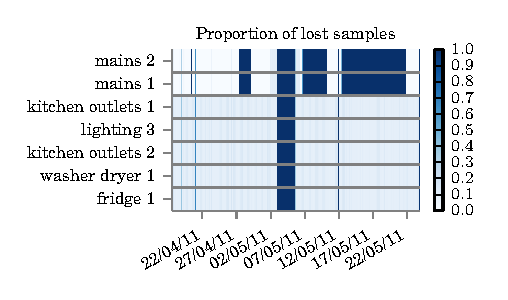
\includegraphics[width=\columnwidth]{figures/lost_samples.pdf} 
  \caption{Lost samples per hour from a representative subset of channels in REDD house 1.}
  \label{fig:lost_samples} 
\end{figure}

\begin{table*}[]
  \centering
\begin{tabular}{cccccc}
\hline
\textbf{Data set} & \textbf{\specialcell[h]{Number of\\appliances}} & \textbf{\specialcell[h]{Percentage\\energy\\sub-metered}} & \textbf{\specialcell[h]{Dropout rate\\(percent)\\ignoring gaps}} & \textbf{\specialcell[h]{Mains up-time\\per house\\(days)}} & \textbf{\specialcell[h]{Percentage\\up-time}} \\
\hline
REDD & 9, 16, 23 &58, 71, 89 & 0, 10, 16 &4, 18, 19 & 8, 40, 79 \\
Smart* &25 & 69 & 6 & 68 & 74 \\
Pecan Street &13, 14, 22 & 75, 87, 150 & 0, 0, 0 &7, 7, 7 & 100, 100, 100 \\
AMPds&20 &97 & 0 &364 & 100 \\
iAWE &10 &48 & 8 & 47 &93 \\
UKPD & 4, 12, 49 &19, 48, 82 &0, 7, 22 & 36, 102, 404 & 73, 84, 100 \\
\hline
\end{tabular}
  \caption{Summary of data set results calculated by the diagnostic and statistical
    functions in NILMTK.  Each cell represents the range of values
    across all households per data set.  The three
    numbers per cell are the minimum, median and maximum values. AMPds, Smart*
    and iAWE each contain just a single house, hence these rows
    have a single number per cell.}
  \label{table:dataset_results}
\end{table*}


\noindent
\tabref{table:dataset_results} shows a selection of diagnostic and statistical functions 
(defined in Section~\ref{sec:diagnostic_definitions} and~\ref{sec:stats_definitions}) computed by NILMTK
across six public data sets. BLUED, Tracebase and HES were not included for the same reasons as in \secref{sec:data_format}. The table illustrates
that AMPds used a robust recording platform because it has a
percentage up-time of 100\%, a dropout rate of zero and 97\% of the
energy recorded by the mains channel was captured by the sub-meters.
Similarly, Pecan Street has an up-time of 100\% and zero dropout rate.  However, two homes
in the Pecan Street data registered a proportion of energy sub-metered of over
100\%. This indicates that some overlap exists between the metered channels, and as a result some appliances are metered by multiple channels.
%despite the removal of channels which were clearly measuring circuits (as distinct from appliances). 
%This indicates that other channels are likely be measuring circuits (and hence some appliances are double-counted). 
%Many data sets do not explicitly describe which sub-meter channels measure circuits and which measure appliances.
%We believe that this is a common problem amongst data sets, and not specific to the Pecan Street data set.
This illustrates the importance of data set metadata (proposed as part
of NILMTK-DF in Section~\ref{sec:data_format}) describing the basic
mains wiring.

Figure~\ref{fig:lost_samples} shows the distribution of missing
samples for REDD house 1.  From this we can see that each mains
recording channel has four large gaps (the solid black blocks) where
the sensors are off and the sub-metered channels have
only one large gap.  Ignoring this gap and focusing on the time
periods where the sensors are recording, we see numerous periods where
the dropout rate is around 10\%.  Such issues are by no means unique
to REDD and are crucial to diagnose before data sets can be used for
the evaluation of disaggregation algorithms or for data set
statistics.

\subsection{Data Set Statistics}

\noindent
Energy disaggregation systems must model individual appliances.  Hence, as well as diagnosing technical issues with each data set, NILMTK also provides functions to visualise patterns of behaviour recorded in each data set. For example, different appliances draw a different amount of power (e.g.\ a toaster draws approximately 1.57~kW), are used at different times of day (e.g.\ the TV is usually on in the evening) and have different correlations with external factors such as weather (e.g.\ lower outside temperature implies more usage of electric heating). Furthermore, load profiles of different appliances of the same type can vary considerably, especially appliances from different countries (e.g.\ the two washing machine profiles in Figure~\ref{fig:wm}). Some disaggregation systems benefit by capturing these patterns (for example, the conditional factorial hidden Markov model (CFHMM)~\cite{kim_2011} can model the influence of time of day on appliance usage). In the following sections, we present examples of how such information can be extracted from existing data sets using NILMTK, covering the distribution of appliance power demands (\secref{sec:power_hist}), usage patterns (\secref{sec:usage_hist}) and external dependencies (\secref{sec:weather_correlation}).

\subsubsection{Appliance power demands}
\label{sec:power_hist}

\noindent
Figure~\ref{fig:power_histograms} displays histograms of the
distribution of powers used by a selection of appliances.  Appliances
such as toasters and kettles tend to have just two possible power states:
on and off.  This simplicity makes them amenable to be modelled by,
for example, Markov chains with only two states per chain.  In contrast, more complex appliances
such as washing machines, vacuum cleaners and computers often
have many more states.

\begin{figure*}[!t]
  \centering
  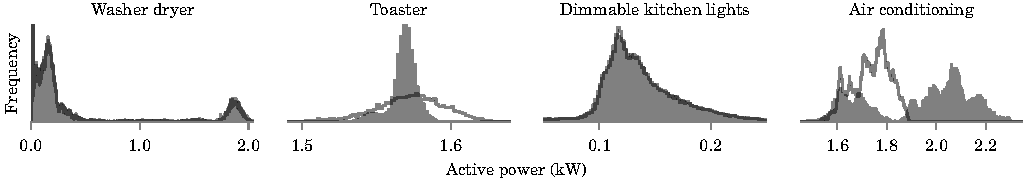
\includegraphics{figures/power_histograms.pdf} 
  \caption{Histograms of power consumption. The filled grey plots show
    histograms of normalised power.  The thin, grey,
    semi-transparent lines drawn over the filled plots show histograms
    of un-normalised power.}
  \label{fig:power_histograms} 
\end{figure*}

Figure~\ref{fig:pie} shows examples of how the proportion of energy use per appliance varies between countries. It can seen that the REDD and UKPD households share some similarities in the breakdown of household energy consumption. In contrast, the iAWE house shows a vastly different energy breakdown. For example, the house recorded in India for the iAWE
data set has two air conditioning units which account for almost half of the household's energy consumption, whilst the example household from the UKPD data set does not even contain an air conditioner.

\begin{figure}
  \centering
  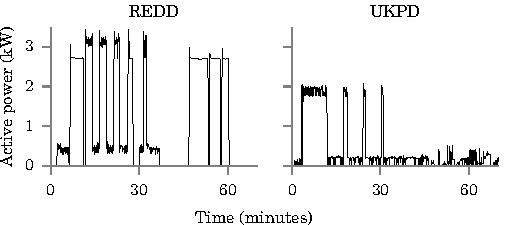
\includegraphics[width=\columnwidth]{figures/wm.pdf}
  \caption{One washing machine from the USA, one from the UK.}
  \label{fig:wm}
\end{figure} 

\begin{figure}[t]
 \centering
 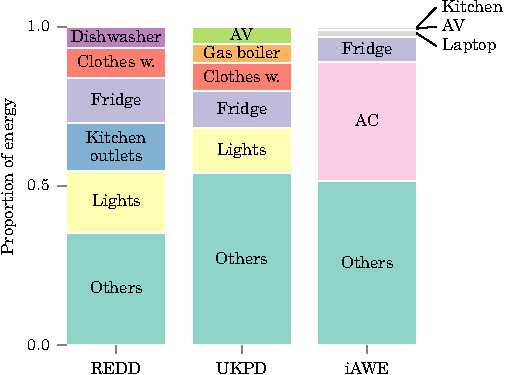
\includegraphics[width=\columnwidth]{figures/top_k_appliances_bar.pdf}
 \caption{Top 5 appliances in terms of the proportion of the total
   energy used in a single house (house 1) in each of REDD (USA), iAWE (India) and
   UKPD (UK).}
 \label{fig:pie}
\end{figure}

%\subsubsection{Learning usage patterns}
%
%\noindent
%A disaggregation system might learn not just to recognise the appearance
%of individual appliances in an aggregate signal but might also learn
%when particular appliances are usually active each day (e.g. the TV is
%usually on in the evening), correlations between appliances (e.g. the
%office LCD screen is on when the office PC is on) and correlations
%between appliances and additional information such as weather data
%from the local meteorological office (e.g. less sunshine implies more
%usage of electric lights).
%
%One probabilistic learning framework capable of capturing this
%information is the conditional factorial hidden Markov model (CFHMM)
%proposed by Kim et. al.~\cite{kim_2011}. They also presented
%several examples of such patterns.  Prior knowledge from
%public datasets could be used to create general probability
%distributions for each appliance class and these distributions could
%then be refined by the disaggregation system for each house.
%
%In the following sections, we present patterns of appliance usage per
%day and per week; correlations between appliance usage and weather
%variables; and histograms of appliance on-durations. 

\subsubsection{Appliance usage patterns}
\label{sec:usage_hist}
\begin{figure}[!t]
  \centering
  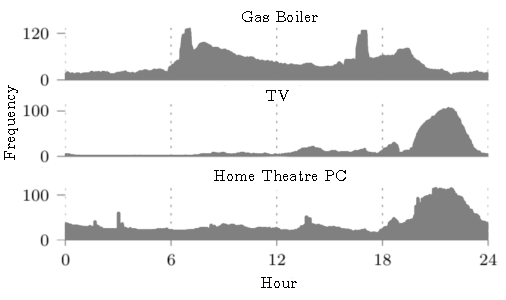
\includegraphics[width=\columnwidth]{figures/daily_usage_histograms3.pdf}
  \caption{Daily appliance usage histograms of three appliances over 120 days from UKPD house 1.}
  \label{fig:daily_usage_histograms}
\end{figure} 

\noindent
%\bluecolor{You may make this subsection of the previous section. Otherwise previous section as a standalong subsection does not look good. Or just give these labels without assigning them sub-sub-sub sections.}
Figure~\ref{fig:daily_usage_histograms} shows histograms which represent usage patterns for three appliances over
an average day, from which strong similarities between groups of appliances can be seen.  For
example, the usage patterns of the TV and Home theatre PC are very
similar because the Home theatre PC is the only video source for the TV. In contrast, the boiler has a usage pattern which occurs as a result of the household's occupancy pattern and hot water timer in mornings and evenings.

\subsubsection{Appliance correlations with weather}
\label{sec:weather_correlation}
\noindent
%We expect the usage of some appliances to be correlated with some weather variables.  
Previous studies have shown correlations
between temperature and heating/cooling demand in
Australia~\cite{RicharddeDear2002} and between temperature and total household demand in the USA~\cite{Kavousian2013a}.  
%We wanted to search for similar correlations.
%If such correlations can be found then a disaggregation system could learn correlations between weather variables and appliance usage in order to refine its appliance usage estimates~\cite{wytock_2013}.\bluecolor{maybe write more succintly Disagg systems can benefit by finding ..correlations}
Such correlations could be used by a NILM system to refine its appliance usage estimates~\cite{wytock_2013}.

Figure~\ref{fig:weather_correlations} shows correlations between
boiler usage and maximum temperature (appliance data from UKPD house 1, temperature data from UK Met Office).  The correlation between
external maximum temperature and boiler usage is strong ($R^2=0.73$) and it is
noteworthy that the $x$-axis intercept ($\approx19\,^{\circ}\mathrm{C}$)
is approximately the set point for the boiler thermostat.

% Lighting circuit usage also correlates with solar radiation
% (not shown) although there is considerable variation in lighting usage
% which is not explained by solar radiation. \bluecolor{should be in appendix if we mention it but don't have space}

\begin{figure}[!t]
  \centering
  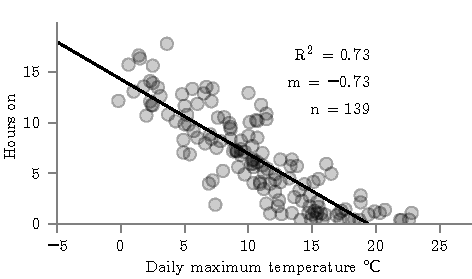
\includegraphics[width=\columnwidth]{figures/weather_correlations2.pdf} 
  \caption{Linear regression showing correlation between gas boiler
    usage and external temperature. $R^2$ denotes the coefficient of
    determination, $m$ is the gradient of the regression line and $n$
    is the number of data-points (days) used in the regression.}
  \label{fig:weather_correlations} 
\end{figure}

\subsection{Voltage Normalisation}

\noindent
%It is inevitable that a household's mains voltage will fluctuate around the nominal value.
%\bluecolor{maybe write better and relate tiwh what we wrote earlier where we gave examples of iawe and smart*} For example, in the UK the nominal mains voltage is 230~V but is allowed to vary by $-6\%,\;{+10}\%$.  This variation in voltage can produce variations in power demand of 20\% in linear loads, such as resistive heaters~\cite{hart_1992}.
%Such abrupt changes in reported power can be problematic for disaggregation algorithms.\bluecolor{rewrite this line}  To mitigate this effect, the power consumption of individual appliances can be normalised as outlined in Section \ref{sec:preprocessing}.
Normalisation can be used to minimise the effect of voltage fluctuations in a household's aggregate power. 
Figure~\ref{fig:power_histograms} shows
histograms for both the normalised and un-normalised appliance power
consumption. Normalisation produces a noticeably tighter power
distribution for linear resistive appliances such as the toaster, although it has
little effect on constant power appliances, such as the washer dryer or LED kitchen ceiling lights. Moreover, on non-linear appliances such as the air conditioner, normalisation increases the variance in power draw. This is in conformance with work by Hart~\cite{hart_1992} which proposed a modified approach to normalisation:
\begin{equation}
\textit{Power}_{\textit{normalised}} = 
\left(\frac{\textit{Voltage}_{\textit{nominal}}}{\textit{Voltage}_{\textit{observed}}}\right)^\beta
\times \textit{Power}_{\textit{observed}}
\end{equation}
For linear appliances such as the toaster, $\beta=2$, whereas for appliances such as fridge, Hart found $\beta=0.7$. Thus, we believe the benefit of voltage normalisation is dependent on the proportion of resistive loads in a household. %(linear)
%that unless a significant proportion of the aggregate load is from resistive (linear) appliances, normalisation may or may not give any improvements in disaggregation performance.

\subsection{Disaggregation Across Data Sets}

\begin{table*}
\centering
\begin{tabular}{ccccccccccc}
\hline\textbf{Data set} & \multicolumn{2}{c}{\textbf{Train time (s)}}& \multicolumn{2}{c}{\textbf{Disaggregate time (s)}} &\multicolumn{2}{c}{\textbf{NEP}}    & \multicolumn{2}{c}{\textbf{FTE}} &\multicolumn{2}{c}{\textbf{F-score}} \\ 
~ &\textbf{CO} & \textbf{FHMM} &\textbf{CO} & \textbf{FHMM} &\textbf{CO} & \textbf{FHMM} &\textbf{CO} & \textbf{FHMM}&\textbf{CO} & \textbf{FHMM} \\ \hline 
REDD &3.67 &22.81 &0.14 &1.21 &1.61 &1.35 &0.77 &0.83 &0.31 &0.31\\ 
Smart* &3.40 &46.34 &0.39 &1.85 &3.10 &2.71 &0.50 &0.66 &0.53 &0.61\\ 
Pecan Street &1.72 &2.83 &0.02 &0.12 &0.68 &0.75 &0.99 &0.87 &0.77 &0.77\\ 
AMPds &5.92 &298.49 &3.08 &22.58 &2.23 &0.96 &0.44 &0.84 &0.55 &0.71\\ 
iAWE &1.68 &8.90 &0.07 &0.38 &0.91 &0.91 &0.89 &0.89 &0.73 &0.73\\ 
UKPD &1.06 &11.42 &0.10 &0.52 &3.66 &3.67 &0.81 &0.80 &0.38 &0.38\\
\hline
\end{tabular}
\caption{Comparison of CO and FHMM across multiple data sets}
\label{table:disaggregation}
\end{table*}

\noindent
We now compare the disaggregation results across the first house of six publicly available data sets. Again, BLUED, Tracebase and HES were not included for the same reasons as in \secref{sec:data_format}. Since all the data sets were collected over different durations, we used the first half of the samples for training and the remaining half for disaggregation across all data sets. Further, we preprocessed  the REDD, UKPD, Smart* and iAWE data sets to 1 minute frequency using the down-sampling filter (\secref{sec:preprocessing}) to account for different aggregate and mains data sampling frequencies and compensating for intermittent lost data packets. The small gaps in REDD, UKPD, SMART* and iAWE were interpolated, while the time periods where either the mains data or appliance data were missing were ignored. AMPds and the Pecan Street data did not require any preprocessing. 
%Apart from REDD, Smart*, UKPD and iAWE, the remaining data sets were processed at the frequency at which they were made available (i.e.\ Pecan Street - 1 minute, AMPds - 1 minute)\bluecolor{already said this?}. 

Since both CO and FHMM have exponential computational complexity in the number of appliances, we model only those appliances whose total energy contribution was greater than 5\%. Across all the data sets, the appliances which contribute more than 5\% of the aggregate include HVAC appliances such as the air conditioner and electric heating, and appliances which are used throughout the day such as the refrigerator. We model all appliances using two states (on and off) across our analyses, although it should be noted that any number of states could be used. However, our experiments are intended to demonstrate a fair comparison of the benchmark algorithms, rather than an fully optimised version of either approach.
%. To the best of our knowledge, there exists no clear solution to the problem of finding the number of states an appliance should be modelled as. While techniques such as elbow joint method for finding the optimum number of clusters and cluster validity measures such as Silhouette measure are similar, we found them to be favouring more states per appliance than what should be expected. 
We compare the disaggregation performance of CO and FHMM across the following three metrics defined in \secref{sec:metrics}: (i) fraction of total energy assigned correctly (FTE), (ii) normalised error in assigned power (NEP) and (iii) F-score. These metrics were chosen because they have been used most often in prior NILM work. Preferable performance is indicated by a low NEP and a high FTE and F-score. The evaluation was performed on a laptop with a 2.3~GHz i7~processor and 8~GB RAM running Linux.

%Table~\tabref{table:disaggregation} summarises the results of the two algorithms across the four data sets. It can be seen that across all the metrics, CO performance is similar to FHMM performance in iAWE and PECAN. In both the used homes from these two datasets, space heating contributes very significantly (about 60\% for a single air conditioner which has a power draw of ~2700 W in the PECAN home and about \redcolor{40\%} across two air conditioner having a power draw of ~1700W and ~1200W respectively. These appliances are easier to disaggregate owing to their huge power demand in comparison to appliances such as electronics and lighting. However, in the first homes used from REDD and AMPds dataset, the power consumption is spread across a lot more number of appliances. A significant number of appliances (14 in AMPds home and 13 in REDD) each contribute less than 5\% of the total load. Under such circumstances, it can be observed that FHMM performance is superior to CO performance across the three metrics. This confirms the theoretical foundations propounded by Hart et al.\cite{hart_1992}; that CO is highly sensitive to small variations in the aggregate load. In contrast, FHMM overcomes these by considering an associated transition probability between states. We further discuss 

\tabref{table:disaggregation} summarises the results of the two algorithms across the six data sets. It can be observed that FHMM performance is superior to CO performance across the three metrics for REDD, Smart* and AMPds. This confirms the theoretical foundations proposed by Hart~\cite{hart_1992}; that CO is highly sensitive to small variations in the aggregate load. The FHMM approach overcomes these shortcomings by considering an associated transition probability between the different states of an appliance. However, it can be seen that CO performance is similar to FHMM performance in iAWE, Pecan Street and UKPD across all metrics. This is likely due to the fact that very few appliances contribute more than 5\% of the household aggregate load in the selected households in these data sets. For instance, space heating contributes very significantly (about 60\% for a single air conditioner which has a power draw of ~2.7 kW in the Pecan Street house and about 35\% across two air conditioners having a power draw of ~1.8 kW and ~1.6 kW respectively in iAWE). As a result, these appliances are easier to disaggregate by both algorithms, owing to their relatively high power demand in comparison to appliances such as electronics and lighting. In the UKPD house the washing machine was one of the appliances contributing more than 5\% of the household aggregate load, which brought down overall metrics across both approaches. 
%\bluecolor{mention circuits are inadequate sometimes! in smart* I suspect this is the case for poor results}
%However, in the first homes used from REDD and AMPds dataset, the power consumption is spread across a lot more number of appliances. A significant number of appliances (14 in AMPds home and 13 in REDD) each contribute less than 5\% of the total load. Under such circumstances,  

Another important aspect to consider is the time required for training and disaggregation, again reported in \tabref{table:disaggregation}. These timings confirm the fact that CO is exponentially quicker than FHMM. This raises an interesting insight: in households such as the ones used from Pecan Street and iAWE in the above analysis, it may be beneficial to use CO over a FHMM owing to the reduced amount of time required for training and disaggregation, even though FHMMs are in general considered to be more powerful. It should be noted that the greater amount of time required to train and disaggregate the AMPds data is a result of the data set containing one year of data, as opposed to the Pecan Street data set which contains one week of data, as shown by \tabref{table:datasets}.

\subsection{Detailed Disaggregation Results}

\tabcolsep=0.14cm
\begin{table}[t]
    \begin{tabular}{ccccc}
    \hline \textbf{Appliance} & \multicolumn{2}{c}{\textbf{NEP}} & \multicolumn{2}{c}{\textbf{F-score}}\\
    ~                  & \textbf{CO}    & \textbf{FHMM}  & \textbf{CO}      & \textbf{FHMM} \\ \hline
    Air conditioner 1  & 0.3   & 0.3   & 0.9     & 0.9  \\
    Air conditioner 2  & 1.0   & 1.0   & 0.7     & 0.7  \\
    Entertainment unit & 4.2   & 4.1   & 0.3     & 0.3  \\
    Fridge             & 0.5   & 0.5   & 0.8     & 0.8  \\
    Laptop computer    & 1.7   & 1.8   & 0.3     & 0.2  \\
    Washing machine    & 130.1 & 125.1 & 0.0     & 0.0  \\
    \hline \end{tabular}
    \caption{Comparison of CO and FHMM across different appliances in iAWE data set}
\label{table:disaggregation_iawe}
\end{table}


\begin{figure}
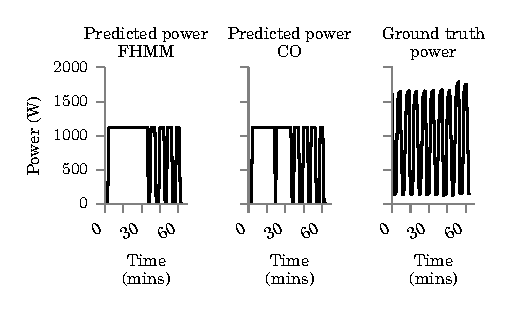
\includegraphics{figures/ac_2.pdf} 
\caption{Comparison of predicted power (CO and FHMM) with ground truth for air conditioner 2 in the iAWE data set}
\label{fig:ac_disaggregation} 
\end{figure}

\noindent
Having compared disaggregation results across different data sets, we now give a detailed discussion of disaggregation results across different appliances for a single house in the iAWE data set. The iAWE data set was chosen for this experiment as the authors provided metadata such as set temperature of air conditioners and other occupant patterns. \tabref{table:disaggregation_iawe} shows the disaggregation performance across the top six energy consuming appliances, in which each appliance is modelled using two states as before. It can be seen that CO and FHMM report similar performance across all appliances. We observe that the results for appliances such as the washing machine and switch mode power supply based appliances such as laptop and entertainment unit (television) are much worse when compared to HVAC loads like air conditioners across both metrics. Furthermore, prior literature shows that complex appliances such as washing machines are hard to model~\cite{barker_2013}.

We observe that the performance accuracy of air conditioner 2 is much worse than air conditioner 1. This is due to the fact that during the instrumentation, air conditioner 2 was operated at a set temperature of $26\,^{\circ}\mathrm{C}$. With an external temperature roughly $5-10\,^{\circ}\mathrm{C}$ below this set temperature, this air conditioner reached the set temperature quickly and turned off the compressor while still running the fan. However, air conditioner 1 was operated at $16\,^{\circ}\mathrm{C}$ and mostly had the compressor on. Thus, air conditioner 2 spent much more time in this intermediate state (compressor off, fan on) in comparison to air conditioner 1. \figref{fig:ac_disaggregation} shows how both FHMM and CO are able to detect on and off events of air conditioner 2. Since air conditioner 2 spent a considerable amount of time in the intermediate state, the learnt two state model is less appropriate in comparison to the two state model used for air conditioner 1. This can be further seen in the figure, where we observe that both FHMM and CO learn a much lower power level of around 1.1~kW, in comparison to the rated power of around 1.6~kW. We believe that this could be corrected by learning a three state model for this air conditioner, which comes at a cost of increased training and disaggregation computational and memory requirements.


\section{Conclusions and future work}
\label{sec:conclusions}

\noindent
In this paper, we proposed NILMTK; the first open source toolkit designed to allow empirical comparisons to be made between energy disaggregation algorithms across multiple data sets. The toolkit defines a common data format, NILMTK-DF, and includes parsers from six publicly available data sets to NILMTK-DF. The toolkit further facilitates the calculation of data set statistics, diagnosing problems and mitigating them via preprocessing functions. In addition, the toolkit includes implementations of two benchmark disaggregation algorithms based on combinatorial optimisation and the factorial hidden Markov model. Finally, NILMTK includes implementations of a set of performance metrics which will enable future research to directly compare disaggregation approaches through a common set of accuracy measures. We demonstrated several analyses facilitated by NILMTK including: use of statistics functions to detect missing data, learning of appliance models from sub-metered data, comparing disaggregation algorithms across multiple data sets and breakdown algorithm performance by individual appliances.

Future work will focus upon the addition of recently proposed training and disaggregation algorithms and data sets. For instance, larger data sets such as HES could also provide additional insight into disaggregation performance.
In addition, recently proposed algorithms which do not require sub-metered power data for their unsupervised training could be compared against the current supervised algorithms.
%These algorithms are computationally expensive so a GPU implementation may be explored. 
% not sure if we should put this as approximate algorithms would be a better solution than CPU implementations
An additional direction for future work could be the use of a semantic wiki to maintain a comprehensive, communal schema for appliance metadata.
%We have made some initial steps towards creating a metadata schema for appliances.  However, we believe the task of maintaining a comprehensive, communal schema may be better suited to a semantic wiki.
Finally, the inclusion of a household simulator (e.g.\ \cite{liang_2010}) would allow disaggregation algorithms to be evaluated in a wider variety of settings than those represented by publicly available data sets.
%Since all data sets represent a limited number of households, it is currently impossible to test how a disaggregation algorithm might perform in a household other than those present in existing data sets. However, a simulator would overcome this problem by generating data for new households by either combining appliance data from multiple households or simulating appliances using detailed appliance models.

%\section{Acknowledgements}

%\noindent
%Nipun Batra would like to thank TCS Research and Development for supporting him through a PhD fellowship and EMC, India for their support. The authors would also like to thank the Department of Electronic and Information Technology (DEITy), Government of India for funding the project (Grant Number DeitY/R\&D/ITEA/4(2)/2012). Jack Kelly would like to thank the EPSRC for his Doctoral Training Account and Intel for their PhD Fellowship grant. 

\bibliographystyle{abbrv}
{\scriptsize
%\begin{small}
\bibliography{reference}
%\end{small}
}

\clearpage
\appendix

%\section{Case Studies}
%\label{sec:use_case}

%\noindent
%In this section we consider two deployment scenarios where NILMTK is being used to perform disaggregation. Firstly, we consider the faculty housing deployment at IIIT Delhi~\cite{batra_2012}. 26 apartments have been instrumented individually with smart meters. Data from these households is being aggregated into a sMAP~\cite{smap} server instance residing inside IIIT Delhi. Aggregate house electricity data from sMAP is pulled via HTTP request and is fed into NILMTK via a converter. The second case study was a single household deployment in Delhi where the data from a Schneider Electric smart meter was collected using a low power Raspberry Pi. In both these cases, rated power of HVAC based appliances such as air conditioners and always on appliances such as refrigerator were used to specify the model. The model was imported using CO disaggregator and disaggregation performed. We created web applications on top of NILMTK for a more engaging user experience. We found that it is trivial to create 3rd party applications on top of NILMTK.

\section{NILMTK-DF}
\label{app:appendix_data_format}
\noindent We now provide the details of NILMTK-DF. \figref{fig:nilmtk-format} shows NILMTK hierarchical structure for modelling physical hierarchies. Each data set consists of one of more households. Each house may comprise of sensors broadly divided as utility (eg. power), ambient (eg. temperature) and external sensors (eg. outside weather). Wherever available, we also store metadata for a household such as area, floor, etc.
Across, utilities, we focus mainly on electrical data, which is divided into mains (coming from grid), panel (circuits) and appliances. Each of these can store multiple physical measurement quantities such as 
active power, voltage etc. Further, wherever available, we also store appliance metadata such as rated power, details of instrumenting sensor, etc. From an implementation perspective, the lowest level in NILMTK-DF hierarchy is stored as a Data Frame, indexed on time and having physical quantities as columns for each of appliances, mains and circuits.
%\begin{figure}
%\centering 
%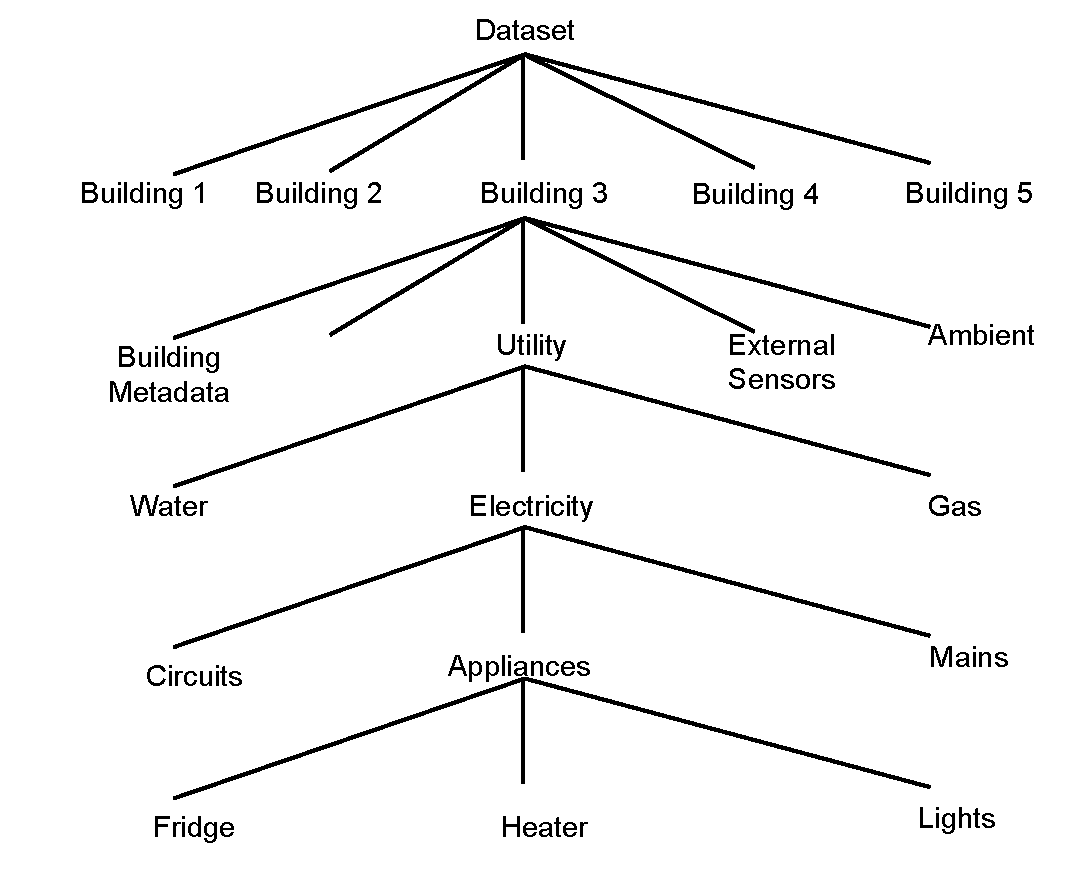
\includegraphics[scale=0.5]{figures/data_format.pdf}
%\caption{NILMTK-DF format hierarchy}
%\label{fig:nilmtk-format}
%\end{figure}
\begin{figure}
\begin{verbatim}
|-- building_1|
|   |-- metadata.json
|   |-- utility
|       |-- electricity
|           |-- appliances
|           |   |-- ac_1.csv
|           |   |-- tv_1.csv
|           |-- appliance_estimates
|           |   |-- estimates_1
|           |       |-- metadata.json
|           |       |-- ac_1.csv
|           |       |-- tv_1.csv
|           |-- circuits
|           |   |-- lights_1.csv
|           |-- mains
|               |-- mains_1_1.csv
|               |-- mains_1_2.csv
|               |-- mains_2_1.csv
|-- building_2
\end{verbatim}
\caption{NILMTK-DF format hierarchy}
\label{fig:nilmtk-format}
\end{figure}

\section{Sample code for NILMTK pipeline}
\label{app:appendix_pipeline}
\noindent We now illustrate the NILMTK pipeline via a minimal code example.

\begin{algorithm}[t]
\begin{verbatim}
dataset = DataSet() 

# Load the dataset
dataset.load_hdf5(DATASET_PATH)

# Load first house
building = dataset.buildings[1]

# Remove records where voltage<160
building = filter_out_implausible_values(
    building, Measurement(`voltage', `'), 160)
    
# Downsample to 1 minute
building = downsample(building, rule=`1T') 

# Choosing feature for disaggregation
DISAGG_FEATURE = Measurement(`power', `active')

# Dividing the data into train and test
train, test = train_test_split(building)

# Train on DISAGG_FEATURES using FHMM 
disaggregator = FHMM() 
disaggregator.train(train, disagg_features=
                   [DISAGG_FEATURE]) 
            
# Disaggregate
disaggregator.disaggregate(test)

# F1 score metric
f1_score = f1(disaggregator.predictions, 
            test) 
\end{verbatim}
 \caption{Example code of complete pipeline.}
 \label{alg:}
\end{algorithm}

\section{Adding a new NILM algorithm}
\label{app:new_algo}
\noindent Every algorithm in NILMTK needs to define the following four functions:
\begin{description}
\item[train]: Parameters of this function are the \texttt{building}; a list of \texttt{disaggregation features} (e.g. \texttt{[active power]} or \texttt{[active power, apparent power]}; 
\texttt{aggregate stream} (e.g. mains) and \texttt{sub-metered stream}(e.g. appliances or circuits)
The parameter style is inspired from R style formulae for linear regression. 
\item[disaggregate]: This function takes as input a \texttt{building} and based on the \texttt{aggregate} and \texttt{sub-metered stream} chosen during training. The output is a disaggregated stream for individual appliances.
\item[import model]: This function should imports from a JSON model to NILMTK disaggregator.
\item[export model]: This function writes the learnt model to a JSON file.
\end{description}

\section{Functions in NILMTK}
\label{app:functions}
In this section we summarise the statistical (\tabref{tab:stats_functions}), diagnostic (\tabref{tab:diagnostic_functions}), and preprocessing (\tabref{tab:preprocessing_functions}) functions in NILMTK. An interested reader may refer the online documentation for updates.
\begin{table}
    \small
    \begin{tabular}{ll}
    \hline
    \textbf{Function} & \textbf{Definition} \\ \hline
    ON-OFF duration       & Finds the distribution of ON-OFF\\
    distribution          &durations of appliances\\ \hline
    Appliance usage       & Finds the temporal distribution\\
    distribution          & of appliance usage\\ \hline
    Appliance power       & Finds the distribution of\\
    distribution          & appliance power draw\\ \hline
    Correlation between   & Finds correlations between\\ 
    sensor streams        & appliances; an appliance \\
                          & and other sensors\\ \hline  
    Find appliance        & Finds contribution of different\\
    contributions         & appliances to the aggregate\\ \hline
    $\%$ energy sub-       & Finds the $\%$ of energy sub-metered\\
    metered               &  by summing up appliance energy and \\
                          &  dividing by mains energy\\ \hline
    $\%$ of samples      & Finds the proportion of samples\\
    when energy sub-  & where the energy sub-metered is \\ 
    metered greater than x &above a threshold\\ \hline
                                                          
    \end{tabular}
    \caption{Statistical functions in NILMTK}
  \label{tab:stats_functions}
\end{table}
 
\begin{table}
    \small
    \begin{tabular}{ll}
    \hline
    \textbf{Function} & textbf{Definition} \\ \hline
    Detect gaps          & Finds gaps between readings which\\
                         & are greater than a threshold\\ \hline
    Find contiguous      & Finds contiguous periods of data\\
    periods              & in sensor data\\ \hline
    Dropout rate         & $\frac{\# \mathrm{Recorded~samples}}{\# \mathrm{Expected~samples}}$\\ \hline
    Dropout rate         & Find the dropout rate ignoring\\
    ignoring large gaps  & large gaps\\ \hline
    Uptime               & Total time for which sensor\\ 
                         & recorded readings\\ \hline
    
    
     
    \end{tabular}
    \caption{Diagnostic functions in NILMTK}
  \label{tab:diagnostic_functions}
\end{table}

\begin{table}
    \small
    \begin{tabular}{ll}
    \hline
    \textbf{Function} & textbf{Definition} \\ \hline
    Voltage               & Given the nominal voltage and\\
    normalisation         &  observed voltage, find normalised\\
                          & power draw as suggested by Hart \\ \hline
    Filter in top-$k$     &Filters in top-$k$ appliances by\\
    appliances            &contribution to aggregate power\\ \hline
    Filter in appliances  &Filters in  only those appliances \\
    contributing above    &which contribute more than $x$\% of\\
    threshold $x$         &aggregate power\\ \hline
    Filter out  impl-     &Removes the readings which are\\
    ausible readings      &outside of a specified range\\ \hline
    Filter out channels   &Removes channels which have \\
    with fewer than $x$   &fewer than $x$ readings \\
    readings              &\\ \hline
    Interpolate           &Interpolates small periods of\\
                          &missing data via forward-filling\\ \hline
    Filter in data between& Excludes data outside the \\
    start and end time    & specified start and end time\\ \hline
    Make common index     &Filters out times where either\\
                          &mains or appliance data is absent\\ \hline
                                                          
    \end{tabular}
    \caption{Preprocessing functions in NILMTK}
  \label{tab:preprocessing_functions}
\end{table}
\section{Query Examples}
\label{app:examples}
We now present some of the wide range of queries supported by NILMTK.

\subsection{Across data sets}
\begin{itemize}
\item How does the daily energy consumption compare across countries?
\item How do instances of an appliance vary across countries?
\item Are there appliances which are country specific?
\end{itemize}

\subsection{Within a data set}
\begin{itemize}
\item How does the power consumption vary over seasons?
\item How does power consumption vary between weekdays and weekend?
\item How does the power consumption of HVAC systems correlate with temperature?
\end{itemize}

%% \section{Appendix2}
%% This section includes content which we currently do not propose to include in the E-Energy paper but which may be included in an extended version of the paper on arXiv.  Or, if our supervisors like any of this content, then we will include it in the main paper.

%% \subsection{Summary of datasets}

%% \subsubsection{Usage histograms}

%% Usage patterns over an average week for the office LCD screen and
%% hoover are shown in figure~\ref{fig:weekly_usage_histograms}.  The
%% office LCD screen is used more frequently on weekdays than on
%% weekends; the inverse is true for the hoover.

%% \begin{figure}[!t]
%%   \centering
%%   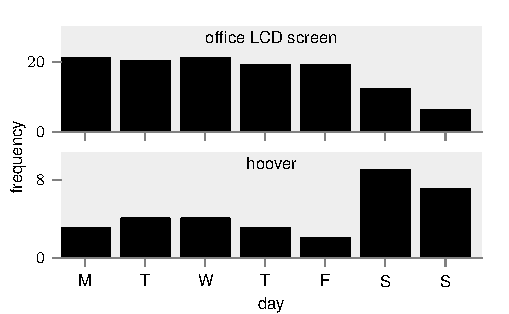
\includegraphics[width=\columnwidth]{figures/weekly_usage_histograms.pdf}
%%   \caption{Weekly appliance usage histograms for the office LCD screen
%%     (top panel) and hoover (bottom panel).  Data from UKPD building 1.}
%%   \label{fig:weekly_usage_histograms}
%% \end{figure}

%% Histograms of on-durations are displayed in
%% figure~\ref{fig:on_durations}. As identified by \cite{kim_2011}, the
%% gamma distribution would be a better fit for several appliance
%% on-durations than the exponential distribution.

%% \begin{figure*}[!t]
%%   \centering
%%   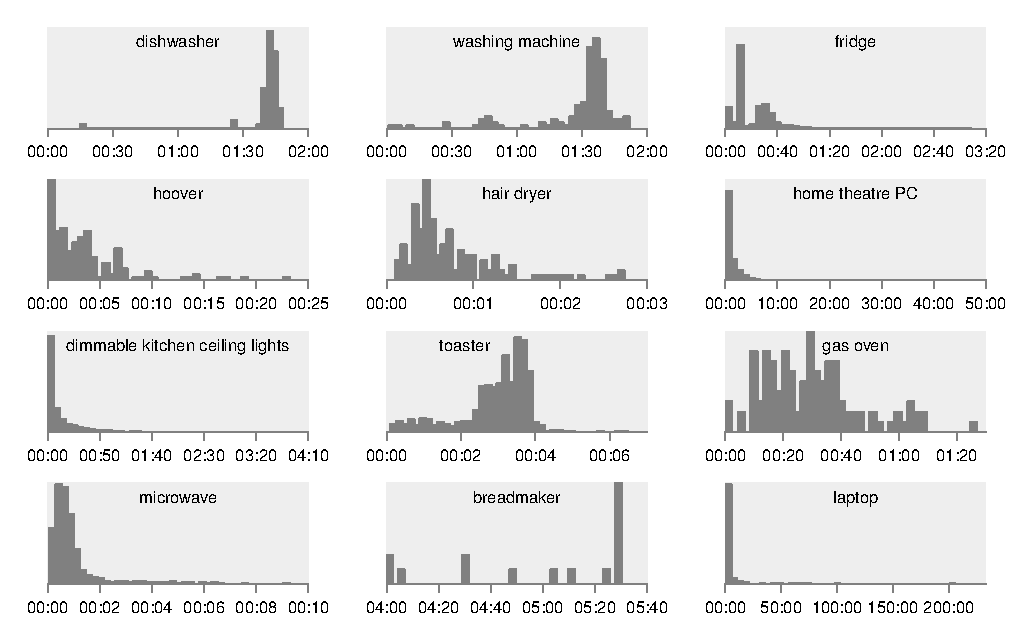
\includegraphics{figures/on_durations.pdf}
%%   \caption{On-durations for a selection of appliances.  The horizontal
%%     axis displays time formatted as ``hours:minutes''.  Outliers have
%%     not been removed.  The laptop was on for over 200 hours (8 days)
%%     while it was being used to collect data.  The home theatre PC was
%%     on for over 40 hours while it was re-installing its operating
%%     system.  Data from UKPD building 1.}
%%   \label{fig:on_durations}
%% \end{figure*}

%% \subsubsection{Correlations with weather}

%% An example of seasonal variation in boiler usage is shown in
%% figure~\ref{fig:seasonal_variation}.  During February, when the
%% weather is relatively cold in the UK, the boiler is primarily used to
%% heat to the radiators for the majority of the day.  In May, when the
%% weather is warmer, the space heating requirement drops away and the
%% twice-daily hot water heating program dominates the usage histogram.

%% \begin{figure}[!t]
%%   \centering
%%   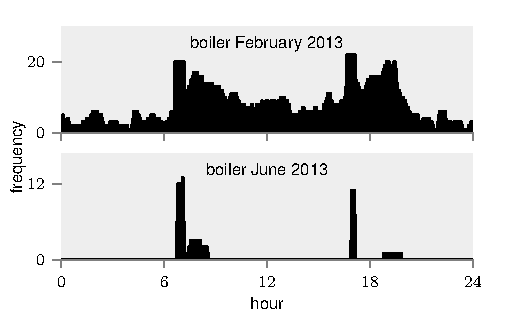
\includegraphics[width=\columnwidth]{figures/seasonal_variation.pdf}
%%   \caption{Seasonal variation in boiler usage.  In June (bottom panel),
%%     the boiler usage histogram is dominated by the hot water program
%%     which runs twice a day.  In February (top panel), considerably
%%     more energy is used on space heating than on hot water heating.   Data from UKPD building 1.}
%%   \label{fig:seasonal_variation}
%% \end{figure}

\end{document}
